\section{Energy integration}


Nasibeh use cetow for heat puming solutions and st fons for large scale integration and combined heat and power production. We have to use neutralised values (i.e. we start with 100 unit and end up with 46.


Converting energy resources into useful energy, exergy efficiency, heat pumping and combined heat and power => examples from the papers of Nasibeh

adding a citation \cite{Pouransari_2014}

testing equations
\begin{equation}
min \, obj= \frac{things_{good}}{things_{bad}} \forall things\\
\text{subject to}  \\
things_{bad}\ge necessary\,\, level \cup unnecessary \, level
\end{equation}

**************

\subsection{Caste study I: Energy integration technologies}

The process heat transfer requirement for a real chemical site is identified using the data collected from different sources including energy conversion, distribution or process units. The heating and cooling requirements have been consequently determined.Based on the heating and cooling requirement definition, the Composite and the Grand Composite Curves are generated in \cref{fig1:mer}. It should be noticed that while defining the energy requirements, we have introduced the streams with the highest possible degree of freedom in order to target the greatest scope for improvement. An individual $\Delta T_{min}$ contribution is considered for each stream by adopting the typical value calculated from a predefined heat exchanger with the film heat transfer coefficient of each fluid at its relevant physical state. The Maximum Energy Recovery (MER) is then determined for the given $\Delta T_{min}$ and is considered as an initial target for heat recovery. \cref{fig1:mer}a shows the maximum heat recovery, the hot and the cold MER. In this case, there is a 54\% potential of integration (from the total heating requirement) compared to 40\% of integration in the current process which corresponds to the first ideal target.


        \begin{figure}[h]
        \begin{center}
        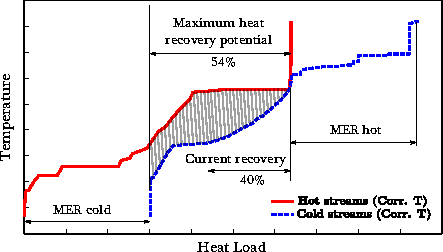
\includegraphics [height=4.3cm]{figures/EnergyIntegration/figMERcc.pdf} 
        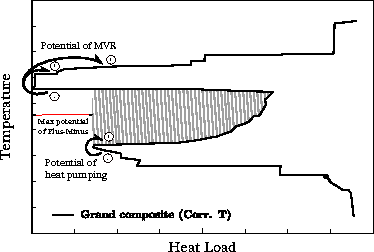
\includegraphics [height=4.3cm]{figures/EnergyIntegration/figMERgcc.pdf}
        \caption{Composite and Grand Composite Curves of the process after heat integration}
        \label{fig1:mer}
        \end{center}
        \end{figure}
        

Based on the result of the GCC and the plus-minus principle \cite{Linnhoff1993503}, the maximum heat recovery can be further improved by either integrating supplementary equipment (like the heat pump) or by modifying process operating conditions (such as modifying the pressure). The analysis of the GCC in \cref{fig1:mer}b with respect to the condition of this system (streams phase and temperature range) shows that there is a large potential for the Mechanical Vapor Recompression (MVR) or heat pumping (or both). The compression cycles are added to the appropriate place with respect to the pinch point temperature. This procedure is however possible until a new pinch point would be activated. Therefore, in order to increase the MVR potential while avoiding a quick creation of new pinch points, the heat pumping system is additionally proposed to be integrated with the Composite Curves. Considering the interdependency of the different actions, the flow rates and the selection of the most effective actions are obtained by solving an optimization problem. Obviously, we bear in mind that the implementation of every new solution of the system will modify the target. Suitable energy conversion units are now integrated and their optimum flow rate is found by Mixed Integer Linear Programming (MILP) formulation proposed by \citet{marechal1998process}. This formulation helps define the heat cascade of the Pinch Analysis method as a set of inequality constraints. This model selects the equipments in the superstructure and determines their optimal operating flow rate in the integrated system. The objective is then to minimize the operating costs, including the fuel and the electricity. In order to optimize the mass flow rates of the MVR, a new equality constraint is also added to the MILP optimization problem. The optimal integration of MVR and heat pumps is performed simultaneously with the energy conversion units. The Composite Curves of the system with MVR alone and together with the heat pumps are respectively shown in \cref{fig1:HPmvr}a and b. By adding an MVR unit, the mechanical power is calculated and a new hot stream is implemented. The principle of the calculation for the MVR is also reported in \cref{fig1:MVR}. In order to create a link between the part which is recompressed and the part used by the direct heat exchange, the equivalent of the expression $\left( \dot{m}_{total}=\dot{m}_{mvr}+\dot{m}_{dhe}\right) $ is added to the MILP problem as a new constraint \cite{EPFL-ARTICLE-163637}.


      \begin{figure}[h]
      \begin{center}
      \begin{tabular}{cc}
        \subfloat[With MVR]{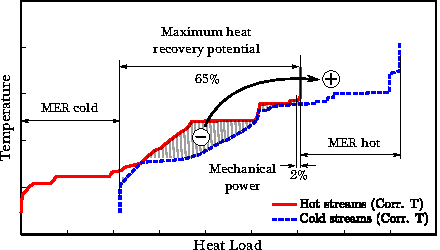
\includegraphics [height=4cm]{figures/EnergyIntegration/HPmvr_mvralone.pdf}} & 
        \subfloat[With MVR and HP]{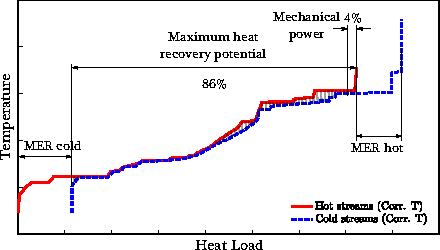
\includegraphics [height=4cm]{figures/EnergyIntegration/HPmvr_mvrhp.pdf}}
       \end{tabular}
      \caption{Composite Curves after improvement potentials}
      \label{fig1:HPmvr}
      \end{center}
      \end{figure}
      
      \begin{figure}[h]
 \begin{center}
 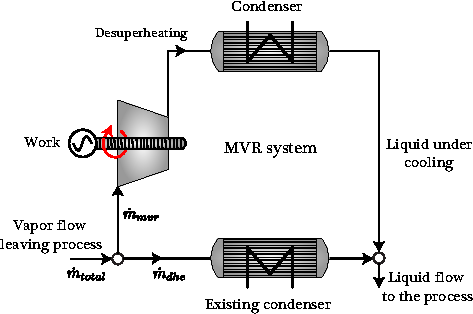
\includegraphics [width=80mm]{images/ch1/MVR.pdf}
 \caption{Principle of the MVR integration}
 \label{fig1:MVR}
 \end{center}
 \end{figure}
 
 Adding an MVR unit to transfer the heat from below to above of the pinch, results in the 11\% further improvement of the heat recovery potential (from 54\% in case of the process integration alone to 65\% in case MVR integrated) at the expense of 2\% mechanical power which corresponds to a COP of 5.5. Considering the newly activated pinch points in \cref{fig1:HPmvr}a, additional heat pumps are also added to system in \cref{fig1:HPmvr}b in order to further increase the heat recovery potential up to 86\%. This results to 32\% additional heat recovery than the original heat integration opportunities including 4\% of mechanical power requirement. This corresponds to a COP of 8. With the three ideal targets shown here, the overall evaluated energy savings could be between 20\% - 45\% approximately.
          
